\section{Design Process or Methodology Overview}

The pipeline has five stages, run independently per model. Stage 1 loads the frozen pretrained model and tokeniser. Stage 2 feeds the 440-stimulus dataset through the model and caches per-layer hidden states. Stage 3 trains per-layer linear probes (one classifier per task per layer) on English and evaluates on both English (in-language) and Bangla (zero-shot cross-lingual transfer). Stage 4 runs surface-feature baselines and stimulus-level sanity checks. Stage 5 runs Representational Similarity Analysis (RSA) and causal forward-hook ablation on the surviving task, with random-unit controls. The same stages run on XLM-R large, Llama 3.1 8B, BLOOM 7B1 and the mT5 XL encoder. Figure~\ref{fig:methodology-pipeline} schematises the end-to-end pipeline; per-model implementations live in \texttt{Dyslexia-XLM-R/main.ipynb}, \texttt{dyslexia-LLM/main.ipynb}, \texttt{dyslexia-bloom/main.ipynb} and \texttt{dyslexia-mt5/main.ipynb} respectively.

\begin{figure}[H]
\centering
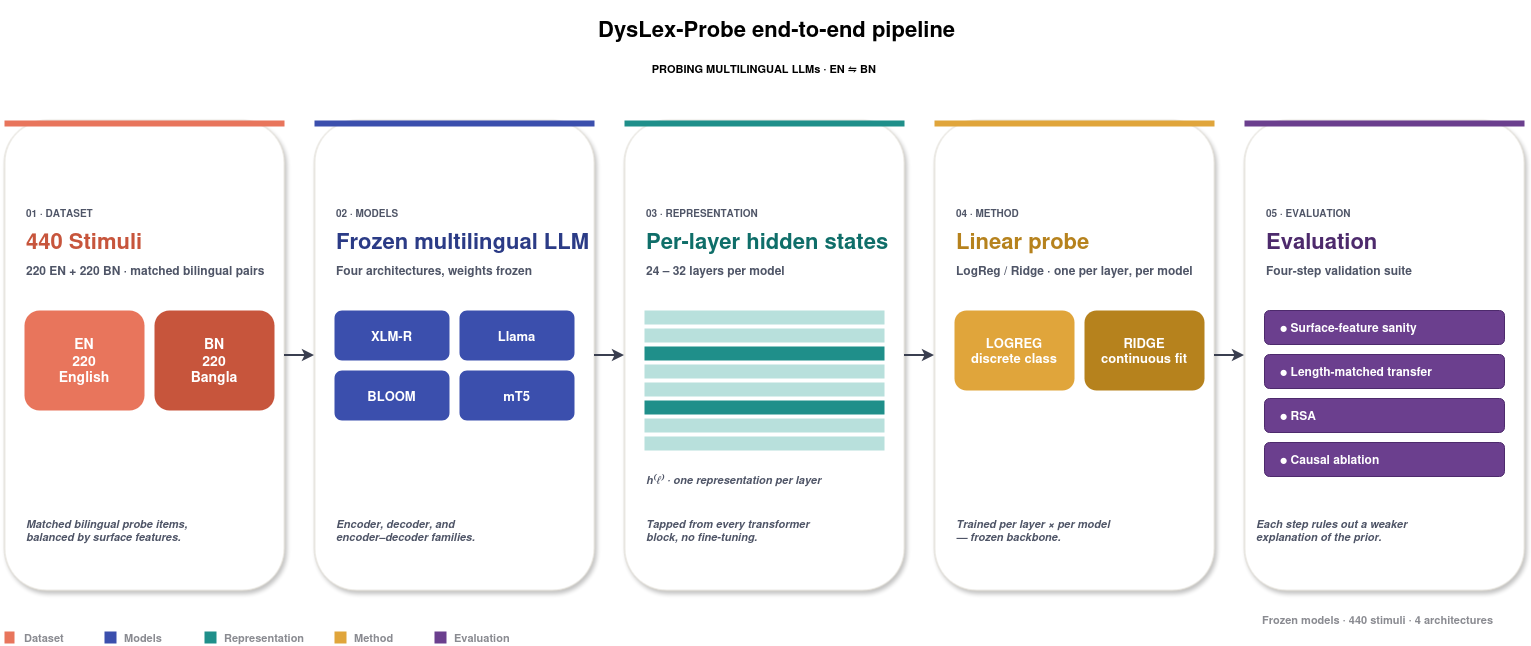
\includegraphics[width=0.95\textwidth]{fig_pipeline.png}
\caption{End-to-end probing pipeline. The 440-stimulus English/Bangla dataset is fed through each frozen multilingual LLM (XLM-R, Llama, BLOOM, mT5); per-layer hidden states are extracted, a linear probe (LogReg/Ridge) is trained, and the resulting representations are evaluated under surface-feature sanity checks, length-matched cross-lingual transfer, Representational Similarity Analysis and causal forward-hook ablation.}
\label{fig:methodology-pipeline}
\end{figure}

\section{Preliminary Design or Design (Model) Specification}

Three design alternatives were considered before settling on frozen per-layer linear probing.

\textbf{Alternative A: Fine-tune each model on each task.} Highest expected performance, but conflates model knowledge with task-specific adaptation, requires large labelled corpora that do not exist for Bangla phonology, and is roughly $10^{6}$ times more expensive in compute than frozen probing. Rejected.

\textbf{Alternative B: Single-layer (final hidden state) probing.} Standard practice in some sentence-level probing studies, but discards information about \emph{where} a feature emerges in the network and prevents the layer-emergence comparison plot (Figure~\ref{fig:layer-emergence}). Rejected.

\textbf{Alternative C (selected): Per-layer linear probing with surface-feature baselines and causal ablation.} Frozen models, linear probes (logistic regression for classification, ridge for regression), per-layer evaluation, length-matched stimulus subsets, RSA and forward-hook ablation. This alternative isolates representational content from model behaviour, exposes layer-wise emergence, and supports causal-localisation claims via random-unit controls. Selected.

\subsection{Models and architectural specification}

Table~\ref{tab:model-specs} summarises the four probed models.

\begin{table}[H]
\centering
\caption{Architectural specification of the four probed multilingual LLMs.}
\label{tab:model-specs}
\small
\resizebox{\textwidth}{!}{%
\setlength{\tabcolsep}{6pt}
\renewcommand{\arraystretch}{2}
\begin{tabular}{|c|c|c|c|c|c|c|}
\hline
\textbf{Model} & \textbf{Architecture} & \textbf{Tokeniser} & \textbf{Params} & \textbf{Layers} & \textbf{Hidden} & \textbf{Bangla coverage} \\
\hline
XLM-R large    & encoder-only         & SentencePiece     & 0.56B            & 24            & 1024 & explicit \\
\hline
Llama 3.1 8B   & decoder-only         & tiktoken BPE      & 8B               & 32            & 4096 & minimal \\
\hline
BLOOM 7B1      & decoder-only         & BPE               & 7.1B             & 30            & 4096 & explicit (ROOTS) \\
\hline
mT5 XL         & encoder-decoder      & SentencePiece     & 3.7B (enc 1.67B) & 24 (encoder)  & 2048 & explicit \\
\hline
\end{tabular}%
}
\end{table}

For mT5 XL only the encoder is probed; the decoder is held frozen and not used for representation extraction. Figure~\ref{fig:model-architectures} compares the four architectures side by side.

\begin{figure}[H]
\centering
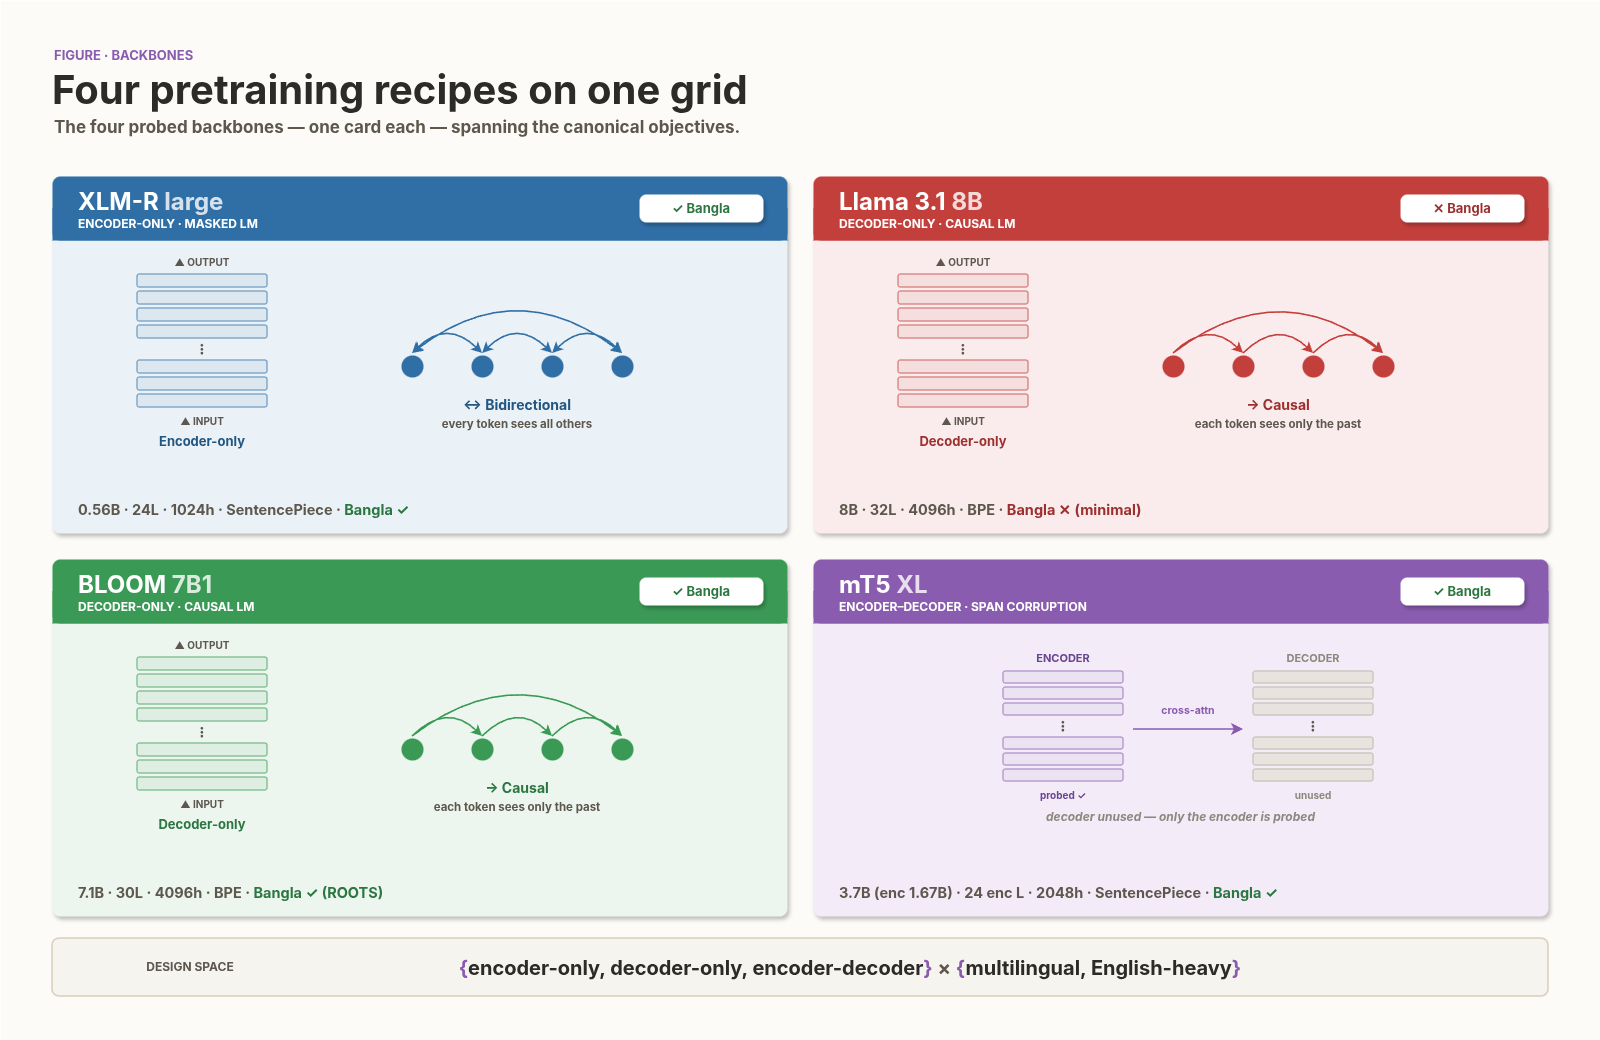
\includegraphics[width=0.98\textwidth]{fig_models.png}
\caption{Side-by-side comparison of the four probed multilingual LLM architectures. XLM-R large is an encoder-only multilingual masked language model; Llama 3.1 8B is an English-heavy causal decoder; BLOOM 7B1 is a 46-language causal decoder with explicit Bangla coverage; mT5 XL is a 101-language span-corruption encoder-decoder. Layer count, hidden size, tokeniser and Bangla coverage are annotated per column.}
\label{fig:model-architectures}
\end{figure}

The four models were selected to exhaust the four canonical pretraining recipes in multilingual NLP as of 2024: a multilingual masked encoder, an English-heavy causal decoder, a multilingual causal decoder, and a multilingual span-corruption encoder-decoder. The following subsections describe each model individually, focusing on the design choices that are most relevant to cross-lingual lexical probing.

\subsection{XLM-RoBERTa large}

XLM-RoBERTa large \cite{conneau2020xlmr} is a 0.56-billion-parameter encoder-only Transformer trained with masked language modelling (MLM) on a 100-language version of the CommonCrawl corpus (CC-100). The model uses a 24-layer encoder stack with hidden dimension 1024 and a SentencePiece tokeniser with a 250{,}000-token vocabulary built jointly across all 100 pretraining languages. Bangla is present in the pretraining mix as an explicitly covered language, and SentencePiece allows Bangla conjunct characters (\textit{yuktoborno}) to be tokenised into subword units rather than discarded. The MLM objective forces the encoder to learn bidirectional contextual representations that integrate information from both left and right context at every position, which is the standard substrate for downstream cross-lingual probing studies \cite{conneau2018probing,hewitt2019structural}. XLM-R large is included here as the representative multilingual MLM-encoder; it is also the smallest model in the comparison, which lets the study quantify how much of cross-lingual lexical transfer can be attributed to multilingual pretraining objective independent of scale.

\textbf{How it works in this study.} Each stimulus (an isolated English or Bangla word) is fed to the model as a single sequence consisting of \texttt{<s>}, the SentencePiece-tokenised word and \texttt{</s>}. A single forward pass in evaluation mode (\texttt{model.eval()}, \texttt{torch.no\_grad()}) returns the 24 layers of hidden states. For each layer the per-token states are mean-pooled across all non-special tokens to a single 1024-dimensional vector, producing a 24-by-1024 representation matrix per stimulus. These vectors are cached to disk under \texttt{Dyslexia-XLM-R/representations/} and consumed by the per-layer probes in the next stage. Because XLM-R is bidirectional, the same forward pass yields representations regardless of token position; no causal-mask correction is needed. The model fits in 16-bit precision on a single 24~GB consumer GPU with no quantisation. Implementation: \texttt{Dyslexia-XLM-R/main.ipynb}.

\subsection{Llama 3.1 8B}

Llama 3.1 8B \cite{dubey2024llama3} is an 8-billion-parameter decoder-only autoregressive Transformer with 32 decoder layers and hidden dimension 4096, trained with a causal language modelling objective on a predominantly English corpus. The tokeniser is a tiktoken-style byte-pair encoding tuned for English with limited explicit coverage of Indic scripts; Bangla characters are handled at the byte level, which is functional but does not group conjuncts as semantic units. Llama 3.1 is the largest and most recent open-weight causal decoder used in this study and represents the dominant industrial recipe of 2024, namely scale-up of a primarily English causal LM. Including it in the comparison is essential precisely because its multilingual coverage is minimal: if any of the cross-lingual lexical signal in this study reflected pure model scale rather than pretraining language coverage, it would surface most clearly in Llama.

\textbf{How it works in this study.} The model is loaded with 4-bit weight quantisation via Unsloth and bitsandbytes \cite{dettmers2022bnb} so that all 32 decoder layers fit on a single 24~GB consumer GPU; activations remain in 16-bit. Each stimulus is fed through the model as a single sequence preceded by the Llama beginning-of-sequence token, with no prompt template. A causal forward pass in evaluation mode yields the 32 layers of hidden states; the causal attention mask means that the state at token position $t$ is conditioned only on tokens up to $t$, so the last token always carries the richest summary in autoregressive use. For consistency with the encoder-based models, however, hidden states for each layer are mean-pooled across all input tokens (excluding the beginning-of-sequence token), producing a 32-by-4096 representation matrix per stimulus. This choice is justified by the probing literature, which finds that mean pooling of decoder hidden states yields more robust linear-probe accuracy than last-token pooling when the downstream task is classification over isolated tokens \cite{conneau2018probing}. Representations are cached under \texttt{dyslexia-LLM/representations/}. Implementation: \texttt{dyslexia-LLM/main.ipynb}.

\subsection{BLOOM 7B1}

BLOOM 7B1 \cite{scao2022bloom} is a 7.1-billion-parameter decoder-only autoregressive Transformer with 30 decoder layers and hidden dimension 4096, trained with a causal language modelling objective on the ROOTS corpus, an explicitly multilingual collection covering 46 natural languages with deliberate over-sampling of low-resource and South-Asian languages including Bangla. The tokeniser is a BPE tokeniser trained jointly across all 46 languages, which means Bangla subword units are first-class citizens of the vocabulary rather than being decomposed at the byte level. BLOOM 7B1 is included as the representative multilingual causal decoder; its pairing with Llama 3.1 8B is the cleanest possible test of whether \emph{multilingual} pretraining of a causal decoder produces transferable cross-lingual lexical structure, because the two models share architecture family and operate at similar parameter scale and differ primarily in pretraining language coverage.

\textbf{How it works in this study.} The pipeline mirrors the Llama pipeline so that any difference in measured cross-lingual transfer is attributable to the pretraining recipe rather than to instrumentation. BLOOM is loaded with 4-bit weight quantisation via Unsloth and bitsandbytes for GPU memory feasibility, with activations in 16-bit. Each stimulus is fed as a single sequence with no prompt template; a single causal forward pass returns the 30 layers of hidden states. Per-layer mean pooling across input tokens (excluding the beginning-of-sequence token) produces a 30-by-4096 representation matrix per stimulus, cached to \texttt{dyslexia-bloom/representations/}. Because BLOOM's BPE tokeniser was trained jointly on Bangla, Bangla input strings decompose into meaningful subword units rather than into raw bytes, and the per-layer mean pool is therefore taken over a smaller and more semantically coherent token sequence than the Llama equivalent. Implementation: \texttt{dyslexia-bloom/main.ipynb}.

\subsection{mT5 XL}

mT5 XL \cite{xue2021mt5} is a 3.7-billion-parameter encoder-decoder Transformer (1.67-billion-parameter encoder) trained with a T5-style span-corruption objective on a 101-language version of the C4 corpus (mC4). The encoder has 24 layers with hidden dimension 2048 and uses a SentencePiece tokeniser shared with the decoder. Bangla is explicitly covered. Span-corruption masks contiguous spans of input tokens and trains the decoder to regenerate them; this objective is qualitatively different from both MLM (which masks individual tokens and reads them off bidirectional context) and causal LM (which never sees right-context at training time), and the resulting encoder representations are organised differently. Critically for this thesis, mT5 is the only encoder-decoder model in the comparison; if the cross-lingual lexical signal turns out to localise differently in mT5 than in the three encoder-only or decoder-only models, the result is interpretable as a property of either the span-corruption objective or the encoder-decoder split, and this is flagged explicitly in the limitations.

\textbf{How it works in this study.} Only the encoder is used. Each stimulus is tokenised with the shared SentencePiece tokeniser and passed through the encoder in evaluation mode; the decoder is loaded but is never invoked during representation extraction. A single forward pass yields the 24 encoder-layer hidden states; per-layer mean pooling over the input tokens produces a 24-by-2048 representation matrix per stimulus, cached to \texttt{dyslexia-mt5/representations/}. The encoder is bidirectional like XLM-R's, so no causal-mask correction is needed. Because the encoder is only 1.67B parameters, mT5 XL fits in 16-bit precision on a single 24~GB consumer GPU without quantisation, which makes mT5 the most expensive but also the highest-fidelity model in the study and is the reason the depth-scan ablation (five \texttt{measure\_L} values, three random-unit seeds each) is run on mT5 specifically and not on the larger BLOOM and Llama decoders. Implementation: \texttt{dyslexia-mt5/main.ipynb}.

\subsection{Why these four}

Each of the four models is the strongest publicly released representative of its pretraining recipe that runs on a single consumer GPU under 4-bit quantisation. Together they span the two-by-two design grid that defines the multilingual LLM landscape in 2024: \{\emph{encoder-only, decoder-only, encoder-decoder}\} crossed with \{\emph{multilingual, English-heavy}\}. Comparing them on the same surface-controlled stimuli with the same probes is the minimal experimental design that lets the thesis make claims about which pretraining recipe carries cross-lingual lexical structure. The four-model comparison is also a precondition for the model-selection recommendation in Chapter~6: without all four families on the same evaluation, it would not be possible to argue that BLOOM is the best practical substrate for a low-resource Bangla screening prototype and that mT5 is the best interpretability substrate.

\section{Data Collection}

\subsection{Stimulus dataset}

The dataset is a single CSV (\texttt{dyslex\_probe\_stimuli\_clean.csv}, 440 rows, 18 columns) committed to each per-model repository. It covers 220 English and 220 Bangla items across seven phonological task categories -- minimal pair (60 per language), multisyllabic (30), pseudoword (25), real word (25), phoneme-grapheme (25), rhyme (20) and sentence (15), totalling 200 items per language -- plus a cross-lingual concept-matching set (20 items per language; 20 translation-equivalent English--Bangla pairs, 40 items total) used for Representational Similarity Analysis, giving 220 items per language and 440 in total. The detailed per-category counts and the eighteen-column schema are reproduced in Appendix~B.

The Bangla side of the stimulus design is grounded in the Master's dissertation work of Badsha \cite{badsha2024mall}, who documented the phonological difficulty patterns of five dyslexic Bangla-speaking primary-school children at the University of Dhaka and published the consolidated findings in IJFMR (vol.\ 6, no.\ 3, May-June 2024). Three elements of our stimulus design are taken directly from that work: (i) the five voiced/unvoiced stop pairs ({\banglafont ক/গ}, {\banglafont প/ব}, {\banglafont ত/দ}, {\banglafont ট/ড}, {\banglafont চ/জ}) used as the Bangla minimal-pair category, (ii) the multisyllabic-word and \textit{matra} error patterns that informed the multisyllabic category, and (iii) the human difficulty ranking (voicing hardest to syllable-count easiest) against which we later compare the four-model ablation pattern in Chapter~5.

Bangla items are stored in Unicode Bengali script with author-assigned IPA, syllable count, phonological complexity, orthographic transparency, voiced/unvoiced label, real-word flag, consonant-cluster flag and irregular-mapping flag. All Bangla items were inspected by a native Bangla speaker for orthographic validity; flagged items were revised or replaced. Bangla pseudowords were generated to follow Bangla phonotactic patterns and re-checked to remove accidental real words.

\subsection{Probing labels}

For each task the label set is:
\begin{itemize}
    \item \textbf{Voicing}: binary \{voiced, unvoiced\}, used on minimal-pair and real-word items where the leading stop consonant has a clear voicing class.
    \item \textbf{Real vs.\ pseudo word (``realword'')}: binary \{real, pseudo\}, used on the union of the real-word and pseudoword categories.
    \item \textbf{Orthographic transparency (``ortho'')}: binary \{transparent, opaque\}, assigned per item from orthographic-mapping rules.
    \item \textbf{Syllable count}: integer regression target.
\end{itemize}

\subsection{Data Cleaning}

Tokeniser-level normalisation differs across model families. To avoid biasing length-based controls, all length statistics (character length, byte length, unique-character count, vowel ratio, consonant-run length) are computed on the original Unicode string before tokenisation, not on the tokeniser output. Bangla conjunct characters (\textit{yuktoborno}) are preserved in their default Unicode encoding; the surface-feature baseline uses the original-string statistics, not the model's subword decomposition.

\subsection{Data Transformation}

For each stimulus the model returns a per-layer sequence of hidden states. For word-level items the per-token states are mean-pooled across the token sequence to a single fixed-dimensional vector per layer per item; for the encoder-decoder model the mean pool is taken over encoder token states only. No normalisation is applied to the pooled vector; probes are trained on the raw pooled hidden state, which is standard in the probing literature \cite{conneau2018probing}.

\subsection{Data Integration}

The hidden-state cache is stored per model in the \texttt{representations/} subdirectory of each per-model repository (one tensor per layer per language). Results from independent model runs are integrated downstream into the comparison files (\texttt{comparison\_three\_models.md} and \texttt{comparison\_four\_models.md}/.xlsx) by joining on (task, layer) keys.

\subsection{Data Reduction}

For the length-matched probing pass (Section~\ref{sec:rq2}), the real-word and pseudoword subsets are reduced to 50 matched pairs per language by selecting 1:1 character-length matches. Mean character length within the matched English subset is 6.88 characters; within the matched Bangla subset, 5.20 characters. This subset is the only one on which length-matched cross-lingual transfer numbers are reported.

\subsection{Summary of Preprocessed Data}

The final analysis-ready dataset is the 440-item stimulus CSV, the per-layer hidden-state caches (one per model), the four label vectors (voicing, realword, ortho, syllable), the 100-item length-matched realword subset (50 EN + 50 BN), and the five-feature character-statistic baseline matrix used in the sanity-check pass.

\section{Implementation of Selected Design}

The full software stack (Python 3.10, PyTorch, Hugging Face \texttt{transformers}, \texttt{scikit-learn}, Unsloth, bitsandbytes, \texttt{matplotlib}, \texttt{pandas} and the pinned version numbers used in this study) and the full hardware specification (single NVIDIA consumer GPU with 24~GB VRAM; 4-bit quantisation for the 7--8B causal decoders) are enumerated in \textbf{Appendix~A: Tools, Software, Hardware and Reproducibility}. The implementation subsections below describe how the design of Chapter~4 is realised in code; readers seeking the exact tool versions, environment files, random seeds and reproducibility checklist should refer to Appendix~A.

\subsection{Representation extraction}

For each model, a single Python notebook loads the frozen pretrained weights via Hugging Face \texttt{transformers}, performs one forward pass per stimulus and writes per-layer mean-pooled hidden states to disk. The Llama and BLOOM models are loaded in 4-bit precision via Unsloth + bitsandbytes \cite{dettmers2022bnb}; XLM-R large and the mT5 encoder fit in 16-bit on a single 24~GB consumer GPU. No model parameters are updated; \texttt{model.eval()} and \texttt{torch.no\_grad()} are enforced throughout.

\subsection{Per-layer probing}

For each (model, layer, task) tuple a fresh probe is trained: L2-regularised logistic regression (scikit-learn, default $C=1.0$) for the three classification tasks, ridge regression (default $\alpha=1.0$) for syllable count. The English subset is split 80/20 (stratified for classification) with \texttt{random\_state=42}. The English-trained probe is evaluated on the held-out English test split (in-language metric) and on the entire Bangla subset (zero-shot cross-lingual transfer metric). Reported metrics are macro F1 for classification and $R^2$ for regression, both averaged over a 5-fold cross-validation within the English training split for layer-selection robustness. Figure~\ref{fig:probing-schematic} illustrates the per-layer probing setup.

\begin{figure}[H]
\centering
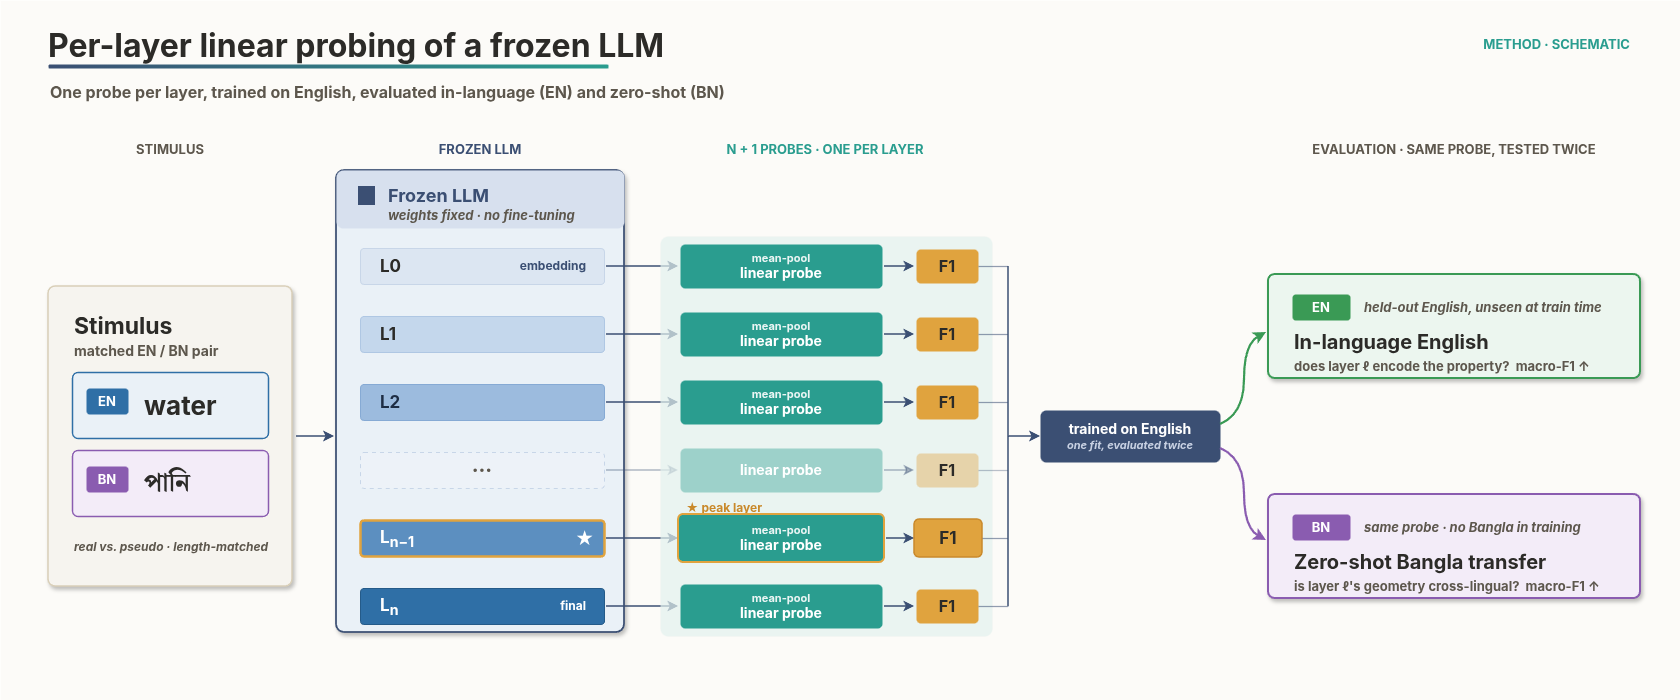
\includegraphics[width=0.85\textwidth]{fig_probing.png}
\caption{Per-layer linear probing schematic. A stimulus passes through the frozen model; each layer's mean-pooled hidden state feeds a separately trained linear probe. The English-trained probe is then evaluated on held-out English (in-language) and on the full Bangla subset (zero-shot cross-lingual transfer).}
\label{fig:probing-schematic}
\end{figure}

\subsection{Surface-feature sanity checks}

Three sanity-check baselines are run.

\textbf{First-character lookup (voicing).} For each Bangla voicing label, the leave-one-out probe is trained on the layer-0 (token-embedding) hidden state with a one-hot encoding of the first character. The resulting F1 quantifies how much voicing information is recoverable from the first character alone (Section~\ref{sec:sanity}, Figure~\ref{fig:bn-voicing-sanity}).

\textbf{Five-feature character-statistic baseline (ortho, syllable).} A logistic / ridge baseline is trained on five hand-crafted features per item: character length, byte length, unique-character count, vowel ratio, longest consonant run. The baseline is run separately for English and Bangla. Any LLM probe whose F1 / $R^2$ does not exceed this baseline by more than 0.03 is interpreted as not contributing information above surface statistics.

\textbf{Length matching (realword).} Real and pseudo word items are matched 1:1 on character length within each language. Probes trained on the matched subset are reported as the only surface-controlled realword numbers.

\subsection{Representational Similarity Analysis}

For each (model, layer) the Representational Dissimilarity Matrix (RDM) over the 220 same-language items is computed using $1 - \cos\theta$ on the mean-pooled hidden states. The English RDM and the Bangla RDM are compared by Spearman $\rho$ on their flattened upper triangles; a high $\rho$ at a layer indicates preserved cross-lingual representational geometry. The mate-retrieval Top-1 accuracy (given an English item, retrieve the matched Bangla item by minimum-cosine-distance) is computed in parallel.

\subsection{Causal forward-hook ablation}

For the length-matched realword task, a probe is first trained on the English baseline at the chosen \texttt{measure\_L} layer (the layer at which transfer is measured). A forward hook is then registered three layers earlier (\texttt{measure\_L - 3}) that, during the forward pass, zeros a chosen subset of hidden units. Two ablation conditions are compared: \textbf{top-$K$} (the $K$ units with the largest absolute probe weights) and \textbf{random-$K$} (a random subset of $K$ units, averaged over three random seeds). The drop in Bangla F1 is reported per condition; \emph{ablation specificity} is defined as (\text{baseline} $-$ \text{top-$K$ accuracy}) $-$ (\text{baseline} $-$ \text{random-$K$ accuracy}). For most reported numbers $K=20$ at the four-model level and $K=10$ at the mT5 depth-scan level. Figure~\ref{fig:ablation-schematic} summarises the design.

\begin{figure}[H]
\centering
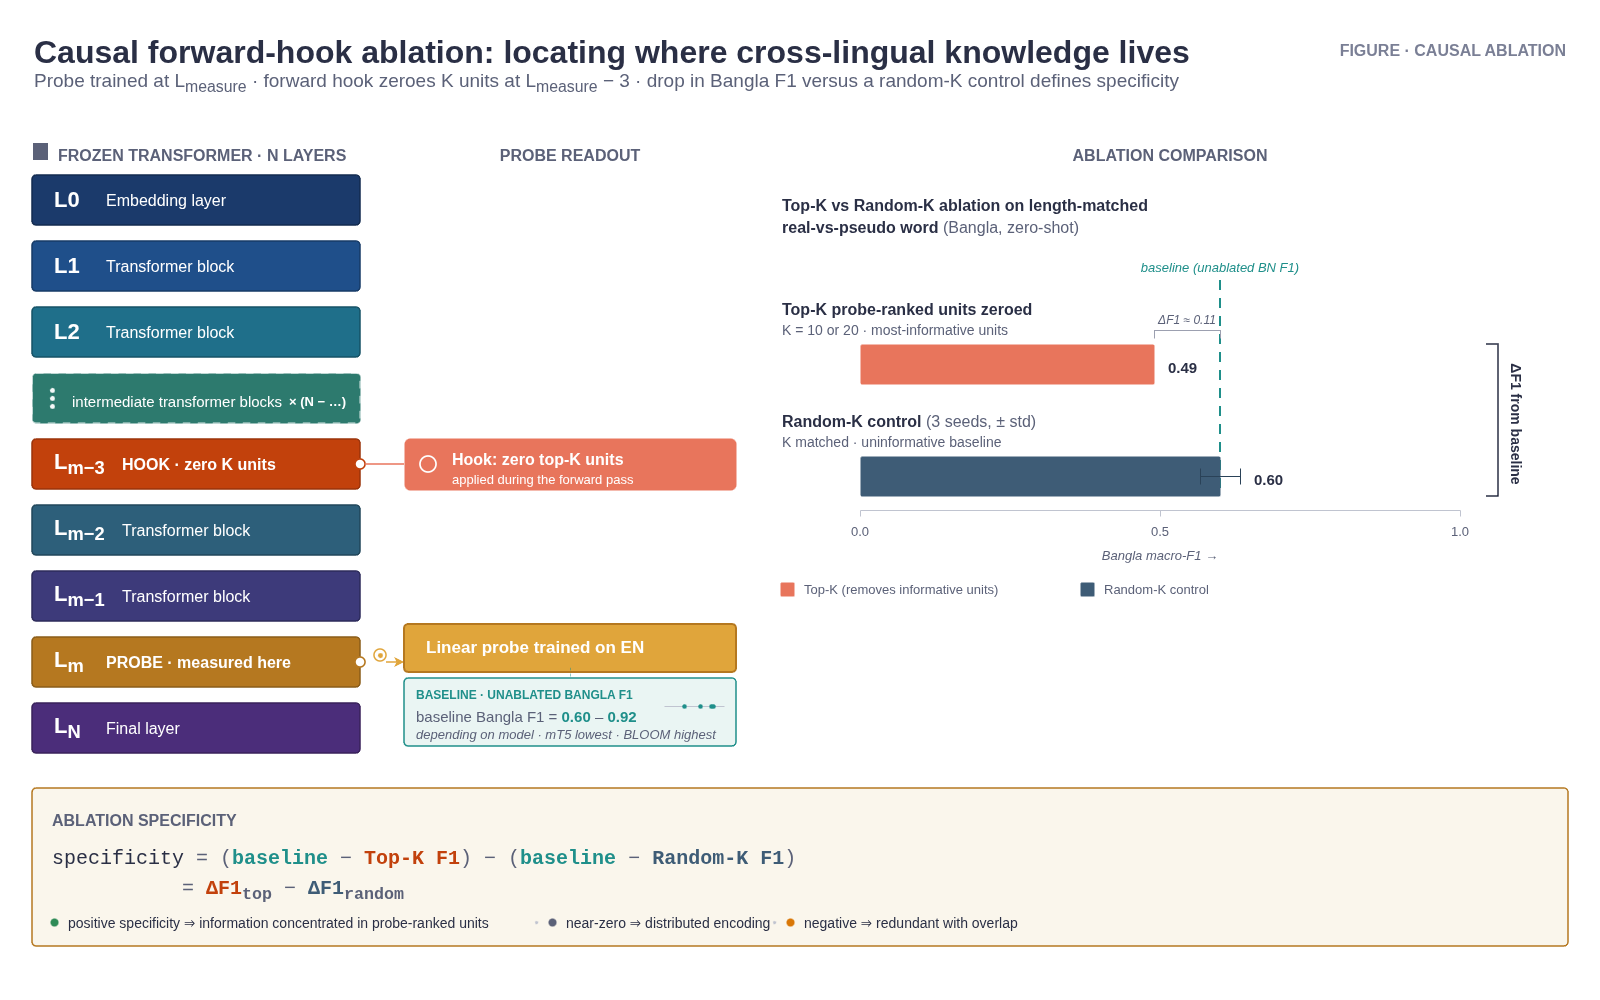
\includegraphics[width=0.95\textwidth]{fig_ablation.png}
\caption{Causal forward-hook ablation. The probe is trained at \texttt{measure\_L}; a forward hook three layers earlier zeros either the top-$K$ probe-ranked units or a random-$K$ control. The drop in Bangla F1 versus the random-$K$ control defines ablation specificity; a positive specificity indicates concentrated, causally relevant units.}
\label{fig:ablation-schematic}
\end{figure}

\subsection{mT5 depth-scan and unit-overlap analysis}

The mT5 encoder ablation is repeated at five depths (\texttt{measure\_L} $\in$ \{4, 8, 12, 16, 20\}) with three random seeds per depth. At each depth the top-10 probe-ranked units are recorded; the pairwise Jaccard overlap of the top-10 sets across depths is then tabulated. A unit that appears in the top-10 at three or more depths is reported as a \emph{persistent backbone} unit; in the mT5 encoder these are u782 and u1880. The analysis answers two questions: (i) does localisation persist across depth or is it specific to one layer; (ii) are the same units carrying the information across depths or does each depth use a layer-local set. Figure~\ref{fig:mt5-backbone-schematic} previews the expected hybrid pattern that the depth-scan ultimately confirms in Chapter~5.

\begin{figure}[H]
\centering
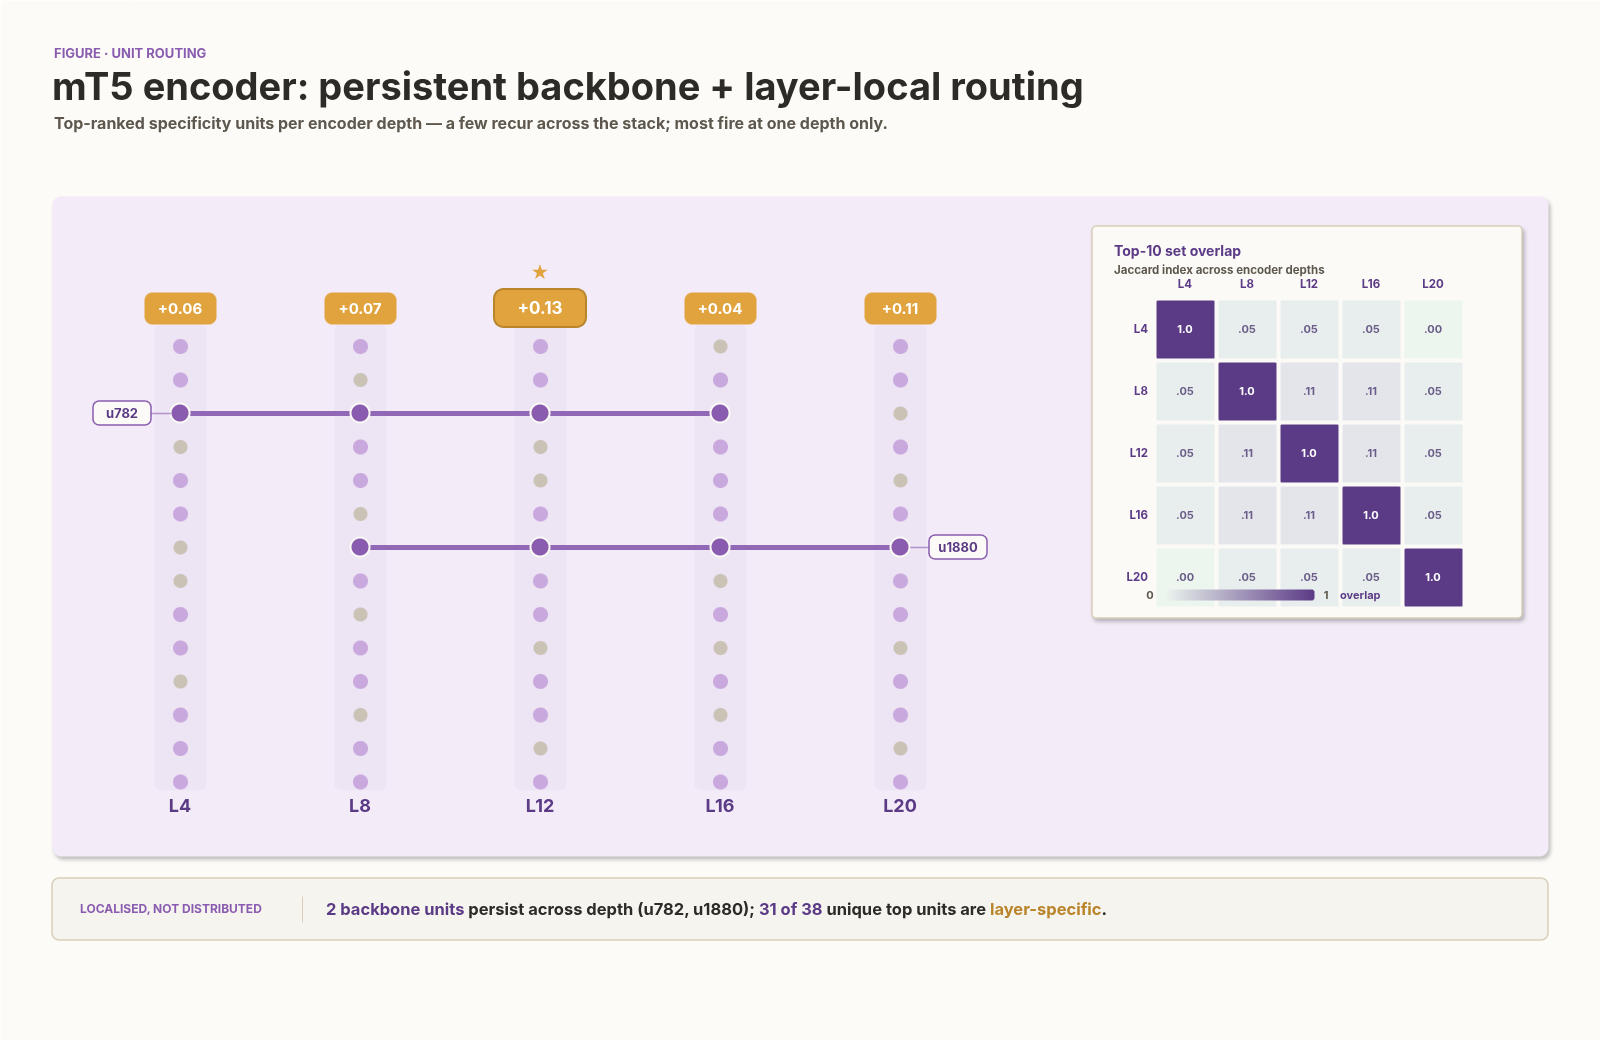
\includegraphics[width=0.95\textwidth]{fig_mt5_backbone.png}
\caption{Schematic of the hybrid backbone-plus-routing pattern probed in the mT5 encoder. Two units (u782, u1880) appear in the top-10 probe-ranked set across four of the five probed encoder depths and constitute a persistent backbone; the remaining top-10 units at each depth are layer-local specialised circuits.}
\label{fig:mt5-backbone-schematic}
\end{figure}

\subsection{Reproducibility}

Every result table in Chapter~5 corresponds to a deterministic CSV in the per-model results directory: \texttt{results\_english\_probing\_*.csv}, \texttt{results\_transfer\_*.csv}, \texttt{results\_rsa\_*.csv}, \texttt{results\_ablation\_*.csv}, \texttt{results\_*\_realword\_matched.csv} and (for mT5) \texttt{results\_mt5\_localization\_depth\_scan.csv} and \texttt{results\_mt5\_unit\_overlap.csv}. Random seeds, scikit-learn versions and CUDA versions are pinned in Appendix~A. The four-model integration is emitted to \texttt{comparison\_four\_models.md} and \texttt{comparison\_four\_models.xlsx} in \texttt{dyslexia-mt5/}.